% ============================================================================
% ENERGY EXPLAIN: FUZZY LOGIC-BASED ENERGY PRICE EXPLAINABILITY SYSTEM
% Complete Project Documentation - Part 1
% ============================================================================

\documentclass[12pt,a4paper]{report}

% ============================================================================
% PACKAGES
% ============================================================================
\usepackage[utf8]{inputenc}
\usepackage[T1]{fontenc}
\usepackage{lmodern}
\usepackage[english]{babel}
\usepackage{amsmath,amssymb,amsfonts}
\usepackage{graphicx}
\usepackage{booktabs}
\usepackage{longtable}
\usepackage{array}
\usepackage{multirow}
\usepackage{xcolor}
\usepackage{listings}
\usepackage{hyperref}
\usepackage{geometry}
\usepackage{fancyhdr}
\usepackage{titlesec}
\usepackage{tocloft}
\usepackage{caption}
\usepackage{subcaption}
\usepackage{float}
\usepackage{algorithm}
\usepackage{algorithmic}
\usepackage{tikz}
\usetikzlibrary{shapes,arrows,positioning,fit,backgrounds}

% ============================================================================
% PAGE SETUP
% ============================================================================
\geometry{
    left=2.5cm,
    right=2.5cm,
    top=2.5cm,
    bottom=2.5cm
}

\pagestyle{fancy}
\fancyhf{}
\fancyhead[L]{\leftmark}
\fancyhead[R]{\thepage}
\renewcommand{\headrulewidth}{0.4pt}

% ============================================================================
% CODE LISTING STYLE
% ============================================================================
\definecolor{codegreen}{rgb}{0,0.6,0}
\definecolor{codegray}{rgb}{0.5,0.5,0.5}
\definecolor{codepurple}{rgb}{0.58,0,0.82}
\definecolor{backcolour}{rgb}{0.95,0.95,0.92}

\lstdefinestyle{pythonstyle}{
    backgroundcolor=\color{backcolour},
    commentstyle=\color{codegreen},
    keywordstyle=\color{magenta},
    numberstyle=\tiny\color{codegray},
    stringstyle=\color{codepurple},
    basicstyle=\ttfamily\footnotesize,
    breakatwhitespace=false,
    breaklines=true,
    captionpos=b,
    keepspaces=true,
    numbers=left,
    numbersep=5pt,
    showspaces=false,
    showstringspaces=false,
    showtabs=false,
    tabsize=2,
    language=Python
}

\lstset{style=pythonstyle}

% ============================================================================
% HYPERREF SETUP
% ============================================================================
\hypersetup{
    colorlinks=true,
    linkcolor=blue,
    filecolor=magenta,
    urlcolor=cyan,
    pdftitle={Energy Explain: Fuzzy Logic Energy Explainability System},
    pdfauthor={},
    pdfsubject={Fuzzy Logic, Energy Markets, Explainable AI},
}

% ============================================================================
% TITLE PAGE
% ============================================================================
\begin{document}

\begin{titlepage}
    \centering
    \vspace*{2cm}
    
    {\Huge\bfseries Energy Explain}\\[0.5cm]
    {\Large\bfseries Fuzzy Logic-Based Energy Price Explainability System}\\[2cm]
    
    {\large Complete Project Documentation}\\[0.5cm]
    {\large Phase 1 \& Phase 2 Implementation Report}\\[3cm]
    
    \vfill
    
    {\large Urban Computing Project}\\[0.5cm]
    {\large December 2025}\\[2cm]
    
    \vfill
\end{titlepage}

% ============================================================================
% TABLE OF CONTENTS
% ============================================================================
\tableofcontents
\newpage

\listoffigures
\listoftables
\newpage

% ============================================================================
% CHAPTER 1: EXECUTIVE SUMMARY
% ============================================================================
\chapter{Executive Summary}

This project presents an advanced \textbf{Fuzzy Logic-Based Energy Price Explainability Dashboard} designed for the Swiss and European energy markets. The system combines \textbf{Mamdani-type Fuzzy Inference Systems (FIS)} with \textbf{Machine Learning (ML)} to provide both numerical predictions and human-interpretable linguistic explanations of energy prices and electricity bills.

The project demonstrates a \textbf{dual explanation paradigm}: numerical analysis for technical users and linguistic reasoning for non-expert consumers, addressing the ``explainability gap'' in modern energy analytics.

\section{Key Features}
\begin{itemize}
    \item Mamdani Fuzzy Inference System with 28 expert-defined rules
    \item Real-time ENTSOE European energy market data integration
    \item Swiss-specific billing analysis with ElCom 2024 tariff rates
    \item Dual explanation system (numerical vs. linguistic)
    \item Interactive Streamlit web dashboard
    \item Linear Regression price prediction with automated feature engineering
\end{itemize}

\section{Project Scope}
\begin{table}[H]
\centering
\caption{Project Statistics}
\begin{tabular}{ll}
\toprule
\textbf{Metric} & \textbf{Value} \\
\midrule
Total Lines of Code & $\sim$5,000+ \\
Number of Modules & 7 core modules \\
Fuzzy Rules & 28 (20 market + 8 recommendation) \\
Input Variables & 5 (price, consumption, hour, volatility, trend) \\
Output Variables & 2 (market\_condition, recommendation) \\
Supported Countries & 17 European nations \\
\bottomrule
\end{tabular}
\end{table}

% ============================================================================
% CHAPTER 2: INTRODUCTION
% ============================================================================
\chapter{Introduction and Problem Statement}

\section{Background}

Energy markets across Europe have experienced unprecedented volatility in recent years, driven by factors including geopolitical tensions, renewable energy integration, and demand fluctuations. Swiss electricity consumers, in particular, face complex billing structures that include:

\begin{itemize}
    \item \textbf{Energy costs}: Actual electricity consumption charges
    \item \textbf{Grid/network charges}: Transmission and distribution fees
    \item \textbf{Taxes and levies}: Cantonal and federal charges
    \item \textbf{Fixed monthly charges}: Base service fees
    \item \textbf{VAT}: 8.1\% Swiss federal tax
\end{itemize}

Understanding why electricity bills vary and how prices are determined remains challenging for most consumers. Traditional analytics tools provide numerical outputs but fail to explain the underlying reasoning in human-understandable terms.

\section{Problem Definition}

This project addresses three critical gaps in current energy analytics:

\begin{enumerate}
    \item \textbf{Lack of Explainability}: Existing energy price prediction systems provide accurate forecasts but cannot explain \textit{why} prices behave a certain way.
    
    \item \textbf{Consumer Confusion}: Complex Swiss billing structures with regional variations make it difficult for consumers to understand their bills.
    
    \item \textbf{Decision Support Gap}: Consumers lack guidance on \textit{when} to consume energy for cost optimization.
\end{enumerate}

\section{Research Objectives}

The primary objectives of this project are:

\begin{enumerate}
    \item Develop a \textbf{Mamdani Fuzzy Inference System} for energy market analysis with linguistic reasoning capabilities
    
    \item Integrate \textbf{real-time ENTSOE data} for accurate European energy market analysis
    
    \item Create a \textbf{Swiss-specific billing analyzer} with canton-level precision
    
    \item Implement a \textbf{dual explanation system} comparing numerical vs. linguistic approaches
    
    \item Build an interactive \textbf{Streamlit dashboard} for real-time analysis and consumer education
\end{enumerate}

% ============================================================================
% CHAPTER 3: THEORETICAL FOUNDATION
% ============================================================================
\chapter{Theoretical Foundation}

\section{Fuzzy Logic Theory}

Fuzzy Logic, introduced by \textbf{Lotfi A. Zadeh in 1965} \cite{zadeh1965}, extends classical Boolean logic to handle partial truth values. Unlike binary logic (true/false), fuzzy logic allows degrees of membership between 0 and 1.

\subsection{Key Concepts}

\subsubsection{Fuzzy Sets}
A fuzzy set $A$ in universe $X$ is characterized by a membership function $\mu_A: X \rightarrow [0,1]$, where $\mu_A(x)$ represents the degree to which element $x$ belongs to set $A$.

\begin{equation}
A = \{(x, \mu_A(x)) | x \in X\}
\end{equation}

For example, ``high price'' is not a crisp threshold but a gradual transition from non-membership to full membership.

\subsubsection{Membership Functions}
This project employs two types of membership functions:

\textbf{Triangular (trimf):} Defined by three parameters $[a, b, c]$:
\begin{equation}
\mu(x; a, b, c) = \max\left(\min\left(\frac{x-a}{b-a}, \frac{c-x}{c-b}\right), 0\right)
\end{equation}

\textbf{Trapezoidal (trapmf):} Defined by four parameters $[a, b, c, d]$:
\begin{equation}
\mu(x; a, b, c, d) = \max\left(\min\left(\frac{x-a}{b-a}, 1, \frac{d-x}{d-c}\right), 0\right)
\end{equation}

\subsubsection{Linguistic Variables}
Variables whose values are words or sentences in natural language. For example:
\begin{itemize}
    \item Variable: \texttt{price}
    \item Linguistic terms: \{very\_low, low, medium, high, very\_high\}
\end{itemize}

\subsubsection{Fuzzy Rules}
IF-THEN statements using linguistic terms:
\begin{verbatim}
IF price IS high AND consumption IS very_high 
THEN market_condition IS unfavorable
\end{verbatim}

\section{Mamdani Fuzzy Inference System}

The \textbf{Mamdani FIS}, introduced by \textbf{Ebrahim Mamdani in 1974} \cite{mamdani1974}, is the most common fuzzy inference methodology.

\subsection{Inference Process}

The Mamdani inference process consists of four steps:

\begin{enumerate}
    \item \textbf{Fuzzification}: Converting crisp inputs to fuzzy membership degrees
    \item \textbf{Rule Evaluation}: Applying fuzzy rules using AND (minimum) and OR (maximum) operators
    \item \textbf{Aggregation}: Combining all rule outputs into a single fuzzy set
    \item \textbf{Defuzzification}: Converting the aggregated fuzzy output back to a crisp value
\end{enumerate}

\subsection{Mathematical Formulation}

For input variables $x_1, x_2, \ldots, x_n$ and output $y$:

\textbf{Rule Evaluation (AND operator - minimum):}
\begin{equation}
\mu_{rule_i}(y) = \min(\mu_{A_1}(x_1), \mu_{A_2}(x_2), \ldots, \mu_{A_n}(x_n))
\end{equation}

\textbf{Aggregation (OR operator - maximum):}
\begin{equation}
\mu_{aggregated}(y) = \max(\mu_{rule_1}(y), \mu_{rule_2}(y), \ldots, \mu_{rule_m}(y))
\end{equation}

\textbf{Defuzzification (centroid method):}
\begin{equation}
y_{crisp} = \frac{\int y \cdot \mu_{aggregated}(y) \, dy}{\int \mu_{aggregated}(y) \, dy}
\end{equation}

\begin{figure}[H]
\centering
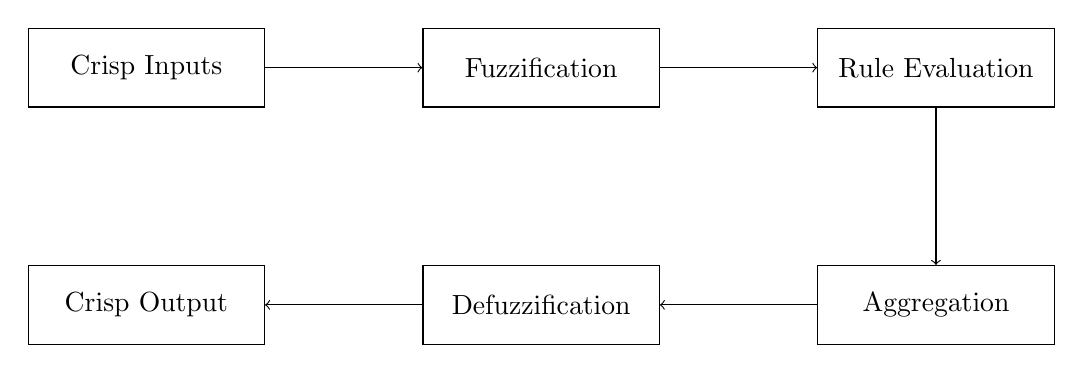
\begin{tikzpicture}[node distance=2cm, auto]
    % Nodes
    \node[draw, rectangle, minimum width=3cm, minimum height=1cm] (input) {Crisp Inputs};
    \node[draw, rectangle, minimum width=3cm, minimum height=1cm, right=of input] (fuzz) {Fuzzification};
    \node[draw, rectangle, minimum width=3cm, minimum height=1cm, right=of fuzz] (rules) {Rule Evaluation};
    \node[draw, rectangle, minimum width=3cm, minimum height=1cm, below=of rules] (agg) {Aggregation};
    \node[draw, rectangle, minimum width=3cm, minimum height=1cm, left=of agg] (defuzz) {Defuzzification};
    \node[draw, rectangle, minimum width=3cm, minimum height=1cm, left=of defuzz] (output) {Crisp Output};
    
    % Arrows
    \draw[->] (input) -- (fuzz);
    \draw[->] (fuzz) -- (rules);
    \draw[->] (rules) -- (agg);
    \draw[->] (agg) -- (defuzz);
    \draw[->] (defuzz) -- (output);
\end{tikzpicture}
\caption{Mamdani Fuzzy Inference Process}
\label{fig:mamdani_process}
\end{figure}

\section{Machine Learning for Price Prediction}

The project employs \textbf{Linear Regression} with automated feature engineering for price prediction. While simpler than deep learning approaches, Linear Regression offers:

\begin{itemize}
    \item \textbf{Interpretability}: Coefficients directly indicate feature importance
    \item \textbf{Transparency}: Decision process is fully explainable
    \item \textbf{Efficiency}: Fast training and inference
    \item \textbf{Baseline Comparison}: Provides benchmark for fuzzy logic evaluation
\end{itemize}

The linear regression model is defined as:
\begin{equation}
\hat{y} = \beta_0 + \beta_1 x_1 + \beta_2 x_2 + \ldots + \beta_n x_n
\end{equation}

where $\beta_i$ are the learned coefficients and $x_i$ are the engineered features.

% ============================================================================
% CHAPTER 4: SYSTEM ARCHITECTURE
% ============================================================================
\chapter{System Architecture}

\section{High-Level Architecture}

The system follows a three-tier architecture consisting of Presentation, Application, and Data layers.

\begin{figure}[H]
\centering
\begin{tikzpicture}[
    layer/.style={draw, rectangle, minimum width=12cm, minimum height=2.5cm, align=center},
    module/.style={draw, rectangle, minimum width=3cm, minimum height=0.8cm, fill=blue!10},
    node distance=0.5cm
]
    % Presentation Layer
    \node[layer, fill=green!10] (pres) {
        \textbf{PRESENTATION LAYER}\\
        Streamlit Dashboard\\[0.3cm]
        \begin{tikzpicture}
            \node[module] at (0,0) {Bill Analysis};
            \node[module] at (4,0) {Price Forecasting};
        \end{tikzpicture}
    };
    
    % Application Layer
    \node[layer, fill=yellow!10, below=of pres] (app) {
        \textbf{APPLICATION LAYER}\\[0.3cm]
        \begin{tikzpicture}
            \node[module] at (0,0) {FuzzyExplainer};
            \node[module] at (3.5,0) {BillingAnalyzer};
            \node[module] at (7,0) {Predictor};
        \end{tikzpicture}
    };
    
    % Data Layer
    \node[layer, fill=red!10, below=of app] (data) {
        \textbf{DATA LAYER}\\[0.3cm]
        \begin{tikzpicture}
            \node[module] at (0,0) {ENTSOE API};
            \node[module] at (3.5,0) {Sample Data};
            \node[module] at (7,0) {CSV Upload};
        \end{tikzpicture}
    };
    
    % Arrows
    \draw[<->] (pres) -- (app);
    \draw[<->] (app) -- (data);
\end{tikzpicture}
\caption{Three-Tier System Architecture}
\label{fig:architecture}
\end{figure}

\section{Module Overview}

\begin{table}[H]
\centering
\caption{System Modules Description}
\label{tab:modules}
\begin{tabular}{llp{6cm}r}
\toprule
\textbf{Module} & \textbf{File} & \textbf{Purpose} & \textbf{LOC} \\
\midrule
Main Application & \texttt{app.py} & Streamlit dashboard with all UI components & 1,660 \\
Fuzzy Explainer & \texttt{fuzzy\_explainer.py} & Mamdani FIS implementation & 1,262 \\
Price Predictor & \texttt{predictor.py} & Linear Regression with feature engineering & 536 \\
Billing Analyzer & \texttt{billing\_analyzer.py} & Swiss bill analysis with ElCom rates & 455 \\
ENTSOE Client & \texttt{entsoe\_client.py} & European energy data API integration & 285 \\
Reason Extractor & \texttt{reason\_extractor.py} & Market insight extraction & 313 \\
Evaluation Manager & \texttt{evaluation\_manager.py} & User feedback persistence & 166 \\
\bottomrule
\end{tabular}
\end{table}

% ============================================================================
% CHAPTER 5: PHASE 1 - CORE IMPLEMENTATION
% ============================================================================
\chapter{Phase 1: Core Implementation}

\section{Fuzzy Inference System}

The core of this project is the Mamdani Fuzzy Inference System implemented in \texttt{fuzzy\_explainer.py}.

\subsection{Input Variables (Antecedents)}

The system defines \textbf{5 input variables} with carefully designed membership functions:

\subsubsection{Price Variable (\texteuro/MWh)}

Universe of discourse: $[0, 200]$

\begin{table}[H]
\centering
\caption{Price Variable Membership Functions}
\begin{tabular}{llp{5cm}}
\toprule
\textbf{Term} & \textbf{Function} & \textbf{Interpretation} \\
\midrule
very\_low & trapmf $[0, 0, 20, 40]$ & Extremely cheap energy \\
low & trimf $[30, 50, 70]$ & Below average prices \\
medium & trimf $[60, 90, 120]$ & Typical market prices \\
high & trimf $[110, 140, 170]$ & Above average prices \\
very\_high & trapmf $[160, 180, 200, 200]$ & Crisis-level prices \\
\bottomrule
\end{tabular}
\end{table}

\subsubsection{Consumption Variable (0-100\% normalized)}

Universe of discourse: $[0, 100]$

\begin{table}[H]
\centering
\caption{Consumption Variable Membership Functions}
\begin{tabular}{llp{5cm}}
\toprule
\textbf{Term} & \textbf{Function} & \textbf{Interpretation} \\
\midrule
very\_low & trapmf $[0, 0, 10, 25]$ & Minimal demand \\
low & trimf $[15, 30, 45]$ & Below average load \\
medium & trimf $[35, 50, 65]$ & Normal demand \\
high & trimf $[55, 70, 85]$ & Peak periods \\
very\_high & trapmf $[75, 90, 100, 100]$ & Maximum grid stress \\
\bottomrule
\end{tabular}
\end{table}

\subsubsection{Hour of Day Variable (0-23)}

Universe of discourse: $[0, 23]$

\begin{table}[H]
\centering
\caption{Hour Variable Membership Functions}
\begin{tabular}{llp{5cm}}
\toprule
\textbf{Term} & \textbf{Function} & \textbf{Interpretation} \\
\midrule
night & trapmf $[0, 0, 4, 6]$ & Lowest demand period \\
morning\_peak & trimf $[6, 8, 10]$ & Commute/startup peak \\
afternoon & trimf $[10, 13, 16]$ & Business hours \\
evening\_peak & trimf $[17, 19, 21]$ & Residential peak \\
late\_evening & trapmf $[20, 22, 23, 23]$ & Declining demand \\
\bottomrule
\end{tabular}
\end{table}

\subsubsection{Volatility Variable (0-50)}

Universe of discourse: $[0, 50]$

\begin{table}[H]
\centering
\caption{Volatility Variable Membership Functions}
\begin{tabular}{llp{5cm}}
\toprule
\textbf{Term} & \textbf{Function} & \textbf{Interpretation} \\
\midrule
low & trapmf $[0, 0, 5, 10]$ & Stable market \\
medium & trimf $[8, 15, 25]$ & Normal fluctuations \\
high & trimf $[20, 30, 40]$ & Elevated uncertainty \\
very\_high & trapmf $[35, 45, 50, 50]$ & Market instability \\
\bottomrule
\end{tabular}
\end{table}

\subsubsection{Trend Variable (-50\% to +50\%)}

Universe of discourse: $[-50, 50]$

\begin{table}[H]
\centering
\caption{Trend Variable Membership Functions}
\begin{tabular}{llp{5cm}}
\toprule
\textbf{Term} & \textbf{Function} & \textbf{Interpretation} \\
\midrule
falling\_fast & trapmf $[-50, -50, -30, -15]$ & Rapid price decrease \\
falling & trimf $[-25, -12, 0]$ & Gradual decrease \\
stable & trimf $[-10, 0, 10]$ & No significant change \\
rising & trimf $[0, 12, 25]$ & Gradual increase \\
rising\_fast & trapmf $[15, 30, 50, 50]$ & Rapid price increase \\
\bottomrule
\end{tabular}
\end{table}

\subsection{Output Variables (Consequents)}

\subsubsection{Market Condition (0-100)}

\begin{table}[H]
\centering
\caption{Market Condition Output Terms}
\begin{tabular}{lp{8cm}}
\toprule
\textbf{Term} & \textbf{Interpretation} \\
\midrule
very\_unfavorable & Consumer should avoid consumption \\
unfavorable & Reduce non-essential usage \\
neutral & Normal market conditions \\
favorable & Good time for consumption \\
very\_favorable & Optimal time for high-load activities \\
\bottomrule
\end{tabular}
\end{table}

\subsubsection{Recommendation (0-100)}

\begin{table}[H]
\centering
\caption{Recommendation Output Terms}
\begin{tabular}{lp{8cm}}
\toprule
\textbf{Term} & \textbf{Interpretation} \\
\midrule
avoid & Do not consume (high prices/peak) \\
reduce & Minimize usage where possible \\
normal & Standard consumption acceptable \\
increase & Favorable for additional usage \\
optimal & Best time for energy-intensive tasks \\
\bottomrule
\end{tabular}
\end{table}

\subsection{Fuzzy Rule Base}

The system implements \textbf{28 fuzzy rules} organized into logical groups.

\subsubsection{Market Condition Rules (20 rules)}

\begin{longtable}{clp{7cm}}
\caption{Market Condition Fuzzy Rules} \\
\toprule
\textbf{ID} & \textbf{Antecedent} & \textbf{Consequent} \\
\midrule
\endfirsthead
\multicolumn{3}{c}{\textit{Continued from previous page}} \\
\toprule
\textbf{ID} & \textbf{Antecedent} & \textbf{Consequent} \\
\midrule
\endhead
\midrule
\multicolumn{3}{r}{\textit{Continued on next page}} \\
\endfoot
\bottomrule
\endlastfoot
1 & price=very\_high $\land$ consumption=very\_high & very\_unfavorable \\
2 & price=very\_high $\land$ consumption=high & very\_unfavorable \\
3 & price=high $\land$ consumption=very\_high & very\_unfavorable \\
4 & price=high $\land$ consumption=high & unfavorable \\
5 & price=very\_low $\land$ consumption=very\_low & very\_favorable \\
6 & price=very\_low $\land$ consumption=low & very\_favorable \\
7 & price=high $\land$ consumption=low & unfavorable \\
8 & price=very\_low $\land$ consumption=high & very\_favorable \\
9 & price=medium $\land$ consumption=medium & neutral \\
10 & hour=night $\land$ price=low & very\_favorable \\
11 & hour=morning\_peak $\land$ price=high & unfavorable \\
12 & hour=evening\_peak $\land$ price=very\_high & very\_unfavorable \\
13 & volatility=very\_high & unfavorable \\
14 & volatility=very\_high $\land$ price=high & very\_unfavorable \\
15 & volatility=low $\land$ price=low & very\_favorable \\
16 & trend=rising\_fast $\land$ price=medium & unfavorable \\
17 & trend=falling\_fast $\land$ price=high $\land$ volatility=low & favorable \\
18 & trend=falling\_fast $\land$ price=high & neutral \\
19 & trend=rising\_fast $\land$ price=low & neutral \\
20 & trend=stable $\land$ price=medium & neutral \\
\end{longtable}

\subsubsection{Recommendation Rules (8 rules)}

\begin{table}[H]
\centering
\caption{Recommendation Fuzzy Rules}
\begin{tabular}{clll}
\toprule
\textbf{ID} & \textbf{Antecedent} & \textbf{Consequent} & \textbf{Purpose} \\
\midrule
R1 & price=very\_low $\land$ hour=night & optimal & Best consumption window \\
R2 & price=low $\land$ consumption=low & optimal & Low demand opportunity \\
R3 & price=very\_high $\land$ hour=evening\_peak & avoid & Worst consumption window \\
R4 & price=high $\land$ hour=morning\_peak & reduce & Peak avoidance \\
R5 & price=medium $\land$ hour=afternoon & normal & Standard operation \\
R6 & price=medium $\land$ consumption=medium & normal & Baseline behavior \\
R7 & price=low $\land$ volatility=low & increase & Stable low prices \\
R8 & price=very\_low $\land$ trend=falling & optimal & Declining price opportunity \\
\bottomrule
\end{tabular}
\end{table}

\subsection{Implementation Code}

\begin{lstlisting}[caption={Fuzzy Variable Definition}, label={lst:fuzzy_vars}]
import numpy as np
import skfuzzy as fuzz
from skfuzzy import control as ctrl

class FuzzyEnergySystem:
    def _setup_input_variables(self):
        # Price variable (EUR/MWh)
        self.price = ctrl.Antecedent(np.arange(0, 201, 1), 'price')
        self.price['very_low'] = fuzz.trapmf(self.price.universe, [0, 0, 20, 40])
        self.price['low'] = fuzz.trimf(self.price.universe, [30, 50, 70])
        self.price['medium'] = fuzz.trimf(self.price.universe, [60, 90, 120])
        self.price['high'] = fuzz.trimf(self.price.universe, [110, 140, 170])
        self.price['very_high'] = fuzz.trapmf(self.price.universe, [160, 180, 200, 200])
        
        # Consumption variable (normalized 0-100)
        self.consumption = ctrl.Antecedent(np.arange(0, 101, 1), 'consumption')
        self.consumption['very_low'] = fuzz.trapmf(self.consumption.universe, [0, 0, 10, 25])
        self.consumption['low'] = fuzz.trimf(self.consumption.universe, [15, 30, 45])
        self.consumption['medium'] = fuzz.trimf(self.consumption.universe, [35, 50, 65])
        self.consumption['high'] = fuzz.trimf(self.consumption.universe, [55, 70, 85])
        self.consumption['very_high'] = fuzz.trapmf(self.consumption.universe, [75, 90, 100, 100])
\end{lstlisting}

\begin{lstlisting}[caption={Fuzzy Rule Definition}, label={lst:fuzzy_rules}]
def _setup_rules(self):
    self.rules = []
    
    # Rule 1: Peak demand crisis
    self.rules.append(ctrl.Rule(
        self.price['very_high'] & self.consumption['very_high'],
        self.market_condition['very_unfavorable']
    ))
    
    # Rule 5: Off-peak optimal
    self.rules.append(ctrl.Rule(
        self.price['very_low'] & self.consumption['very_low'],
        self.market_condition['very_favorable']
    ))
    
    # Rule 10: Night advantage
    self.rules.append(ctrl.Rule(
        self.hour['night'] & self.price['low'],
        self.market_condition['very_favorable']
    ))
\end{lstlisting}

\begin{lstlisting}[caption={Fuzzy Evaluation Function}, label={lst:fuzzy_eval}]
def evaluate(self, price_value, consumption_value, hour_value, 
             volatility_value=10, trend_value=0):
    """
    Evaluate the fuzzy inference system with given inputs.
    """
    results = {
        'market_condition': 50,
        'recommendation': 50,
        'memberships': {},
        'active_rules': []
    }
    
    # Clip values to valid universe ranges
    price_value = np.clip(float(price_value), 0, 200)
    consumption_value = np.clip(float(consumption_value), 0, 100)
    hour_value = np.clip(int(hour_value), 0, 23)
    
    # STEP 1: FUZZIFICATION
    results['memberships'] = {
        'price': self._get_membership_degrees(self.price, price_value),
        'consumption': self._get_membership_degrees(self.consumption, consumption_value),
        'hour': self._get_membership_degrees(self.hour, hour_value)
    }
    
    # STEP 2-4: INFERENCE AND DEFUZZIFICATION
    self.market_sim.input['price'] = price_value
    self.market_sim.input['consumption'] = consumption_value
    self.market_sim.input['hour'] = hour_value
    self.market_sim.compute()
    
    results['market_condition'] = float(self.market_sim.output['market_condition'])
    
    return results
\end{lstlisting}

\section{Price Prediction Module}

\subsection{Feature Engineering}

The predictor implements \textbf{automated feature engineering} creating the following features from raw datetime and consumption data:

\subsubsection{Cyclical Temporal Features}

To preserve the cyclical nature of time, sine and cosine transformations are applied:

\begin{align}
\text{hour\_sin} &= \sin\left(\frac{2\pi \times \text{hour}}{24}\right) \\
\text{hour\_cos} &= \cos\left(\frac{2\pi \times \text{hour}}{24}\right) \\
\text{dow\_sin} &= \sin\left(\frac{2\pi \times \text{day\_of\_week}}{7}\right) \\
\text{dow\_cos} &= \cos\left(\frac{2\pi \times \text{day\_of\_week}}{7}\right) \\
\text{month\_sin} &= \sin\left(\frac{2\pi \times \text{month}}{12}\right) \\
\text{month\_cos} &= \cos\left(\frac{2\pi \times \text{month}}{12}\right)
\end{align}

\subsubsection{Binary Features}
\begin{itemize}
    \item \texttt{is\_weekend}: Saturday or Sunday indicator
    \item \texttt{is\_peak\_hour}: Hours 7-9 or 18-21 indicator
\end{itemize}

\subsubsection{Polynomial Features}
\begin{itemize}
    \item \texttt{consumption\_squared}: Non-linear consumption effects
\end{itemize}

\subsubsection{Lag Features}
\begin{itemize}
    \item \texttt{consumption\_lag\_1}: Previous hour consumption
    \item \texttt{consumption\_lag\_24}: Same hour yesterday
    \item \texttt{price\_lag\_1}: Previous hour price
    \item \texttt{price\_lag\_24}: Same hour yesterday price
\end{itemize}

\subsubsection{Rolling Statistics}
\begin{itemize}
    \item \texttt{consumption\_rolling\_mean\_24}: 24-hour rolling average
    \item \texttt{consumption\_rolling\_std\_24}: 24-hour rolling standard deviation
\end{itemize}

\subsection{Model Implementation}

\begin{lstlisting}[caption={Price Predictor Implementation}, label={lst:predictor}]
from sklearn.linear_model import LinearRegression
from sklearn.model_selection import train_test_split
from sklearn.metrics import mean_absolute_error, mean_squared_error, r2_score

class EnergyPricePredictor:
    def __init__(self):
        self.model = LinearRegression()
        self.is_trained = False
        
    def create_features(self, df):
        """Create automated features from raw data."""
        df_features = df.copy()
        
        # Cyclical encoding
        df_features['hour_sin'] = np.sin(2 * np.pi * df['hour'] / 24)
        df_features['hour_cos'] = np.cos(2 * np.pi * df['hour'] / 24)
        
        # Binary features
        df_features['is_weekend'] = df['day_of_week'].isin([5, 6]).astype(int)
        df_features['is_peak_hour'] = df['hour'].apply(
            lambda x: 1 if (7 <= x <= 9) or (18 <= x <= 21) else 0
        )
        
        # Lag features
        df_features['consumption_lag_1'] = df['energy_consumption'].shift(1)
        df_features['consumption_lag_24'] = df['energy_consumption'].shift(24)
        
        return df_features.dropna()
    
    def train(self, df, target_column='price', test_size=0.2):
        """Train the linear regression model."""
        df_features = self.create_features(df)
        
        X = df_features[self.feature_names].values
        y = df_features[target_column].values
        
        self.X_train, self.X_test, self.y_train, self.y_test = train_test_split(
            X, y, test_size=test_size, random_state=42
        )
        
        self.model.fit(self.X_train, self.y_train)
        self.is_trained = True
        
        return self
\end{lstlisting}

\subsection{Performance Metrics}

The model computes three key metrics:

\begin{itemize}
    \item \textbf{MAE (Mean Absolute Error)}: Average prediction error in \texteuro/MWh
    \begin{equation}
    \text{MAE} = \frac{1}{n}\sum_{i=1}^{n}|y_i - \hat{y}_i|
    \end{equation}
    
    \item \textbf{RMSE (Root Mean Squared Error)}: Error penalizing large deviations
    \begin{equation}
    \text{RMSE} = \sqrt{\frac{1}{n}\sum_{i=1}^{n}(y_i - \hat{y}_i)^2}
    \end{equation}
    
    \item \textbf{R² Score}: Coefficient of determination
    \begin{equation}
    R^2 = 1 - \frac{\sum_{i=1}^{n}(y_i - \hat{y}_i)^2}{\sum_{i=1}^{n}(y_i - \bar{y})^2}
    \end{equation}
\end{itemize}

\section{ENTSOE Data Integration}

\subsection{Supported Countries}

The ENTSOE client supports \textbf{17 European countries/regions}:

\begin{table}[H]
\centering
\caption{ENTSOE Supported Countries}
\begin{tabular}{ll|ll}
\toprule
\textbf{Country} & \textbf{Domain Code} & \textbf{Country} & \textbf{Domain Code} \\
\midrule
Germany & 10Y1001A1001A83F & France & 10YFR-RTE------C \\
Switzerland & 10YCH-SWISSGRIDZ & Austria & 10YAT-APG------L \\
Belgium & 10YBE----------2 & Netherlands & 10YNL----------L \\
Italy (North) & 10Y1001A1001A73I & Spain & 10YES-REE------0 \\
Portugal & 10YPT-REN------W & Poland & 10YPL-AREA-----S \\
Czech Republic & 10YCZ-CEPS-----N & Denmark & 10Y1001A1001A65H \\
Norway & 10YNO-0--------C & Sweden & 10YSE-1--------K \\
Finland & 10YFI-1--------U & Great Britain & 10YGB----------A \\
Ireland & 10Y1001A1001A59C & & \\
\bottomrule
\end{tabular}
\end{table}

\subsection{Data Types Retrieved}

\begin{enumerate}
    \item \textbf{Day-Ahead Prices (A44)}: Hourly prices for next-day delivery
    \item \textbf{Actual Prices (A25)}: Real-time settlement prices
    \item \textbf{Actual Load (A65)}: Real-time grid demand
\end{enumerate}

\subsection{API Implementation}

\begin{lstlisting}[caption={ENTSOE Client Implementation}, label={lst:entsoe}]
import requests
from datetime import datetime, timedelta

class ENTSOEClient:
    BASE_URL = "https://web-api.tp.entsoe.eu/api"
    
    DOMAINS = {
        'Germany': '10Y1001A1001A83F',
        'France': '10YFR-RTE------C',
        'Switzerland': '10YCH-SWISSGRIDZ',
        # ... other countries
    }
    
    def __init__(self, api_token):
        self.api_token = api_token
    
    def fetch_complete_dataset(self, country, days=7):
        """Fetch prices and load data for specified country."""
        end_date = datetime.now()
        start_date = end_date - timedelta(days=days)
        
        prices_df = self._fetch_day_ahead_prices(country, start_date, end_date)
        load_df = self._fetch_actual_load(country, start_date, end_date)
        
        merged = pd.merge(prices_df, load_df, on='datetime', how='inner')
        merged.columns = ['datetime', 'price', 'energy_consumption']
        
        return merged
    
    def _fetch_day_ahead_prices(self, country, start, end):
        """Fetch day-ahead prices from ENTSOE."""
        params = {
            'securityToken': self.api_token,
            'documentType': 'A44',
            'in_Domain': self.DOMAINS[country],
            'out_Domain': self.DOMAINS[country],
            'periodStart': start.strftime('%Y%m%d%H%M'),
            'periodEnd': end.strftime('%Y%m%d%H%M')
        }
        response = requests.get(self.BASE_URL, params=params)
        return self._parse_price_xml(response.content)
\end{lstlisting}

% End of Part 1
% Continue in Part 2...

\end{document}
